\documentclass[aspectratio=169]{ctexbeamer} % normal mode:& for lecturing 
% \documentclass[aspectratio=169, draft]{ctexbeamer} % draft mode:& to compile faster 
% \documentclass[aspectratio=169, handout]{ctexbeamer} % handout mode:& when releasing slides 
% \setbeamertemplate{footline}[frame number] % use this when releasing pdf
\usepackage{amsmath}
\usepackage{booktabs}
\usepackage{graphicx}
\usepackage{ulem}
\usepackage{xcolor}
\hypersetup{colorlinks}
\setbeamertemplate{caption}{\raggedright\insertcaption\par}
% \setbeamercovered{transparent}

% \AtBeginSection[]
% {
% \begin{frame}
%     \frametitle{}
%     \tableofcontents[currentsection]
% \end{frame}
% }
% TODO: fill title here
\title{Final project: 用两个三角形渲染世界}
\author{张高阳}
% \date{Feb 23 2020}

\begin{document}
\begin{frame}
    \titlepage 
\end{frame}

\begin{frame}
    \frametitle{简介}
    \begin{columns}
        \begin{column}{.1\textwidth}\end{column}
        \begin{column}{.5\textwidth}
            \begin{itemize}
                \item 选题: \underline{2.4.2}: 用两个三角形渲染世界
                \item 冰淇淋 \texttt{emoji}
            \end{itemize}
        \end{column}
        \begin{column}{.4\textwidth}
            
\includegraphics[width=32pt]{images/pre/emoji.pdf}
        \end{column}
    \end{columns}
\end{frame}

\begin{frame}
    \frametitle{效果}
    \begin{figure}[htbp]
        \centering
        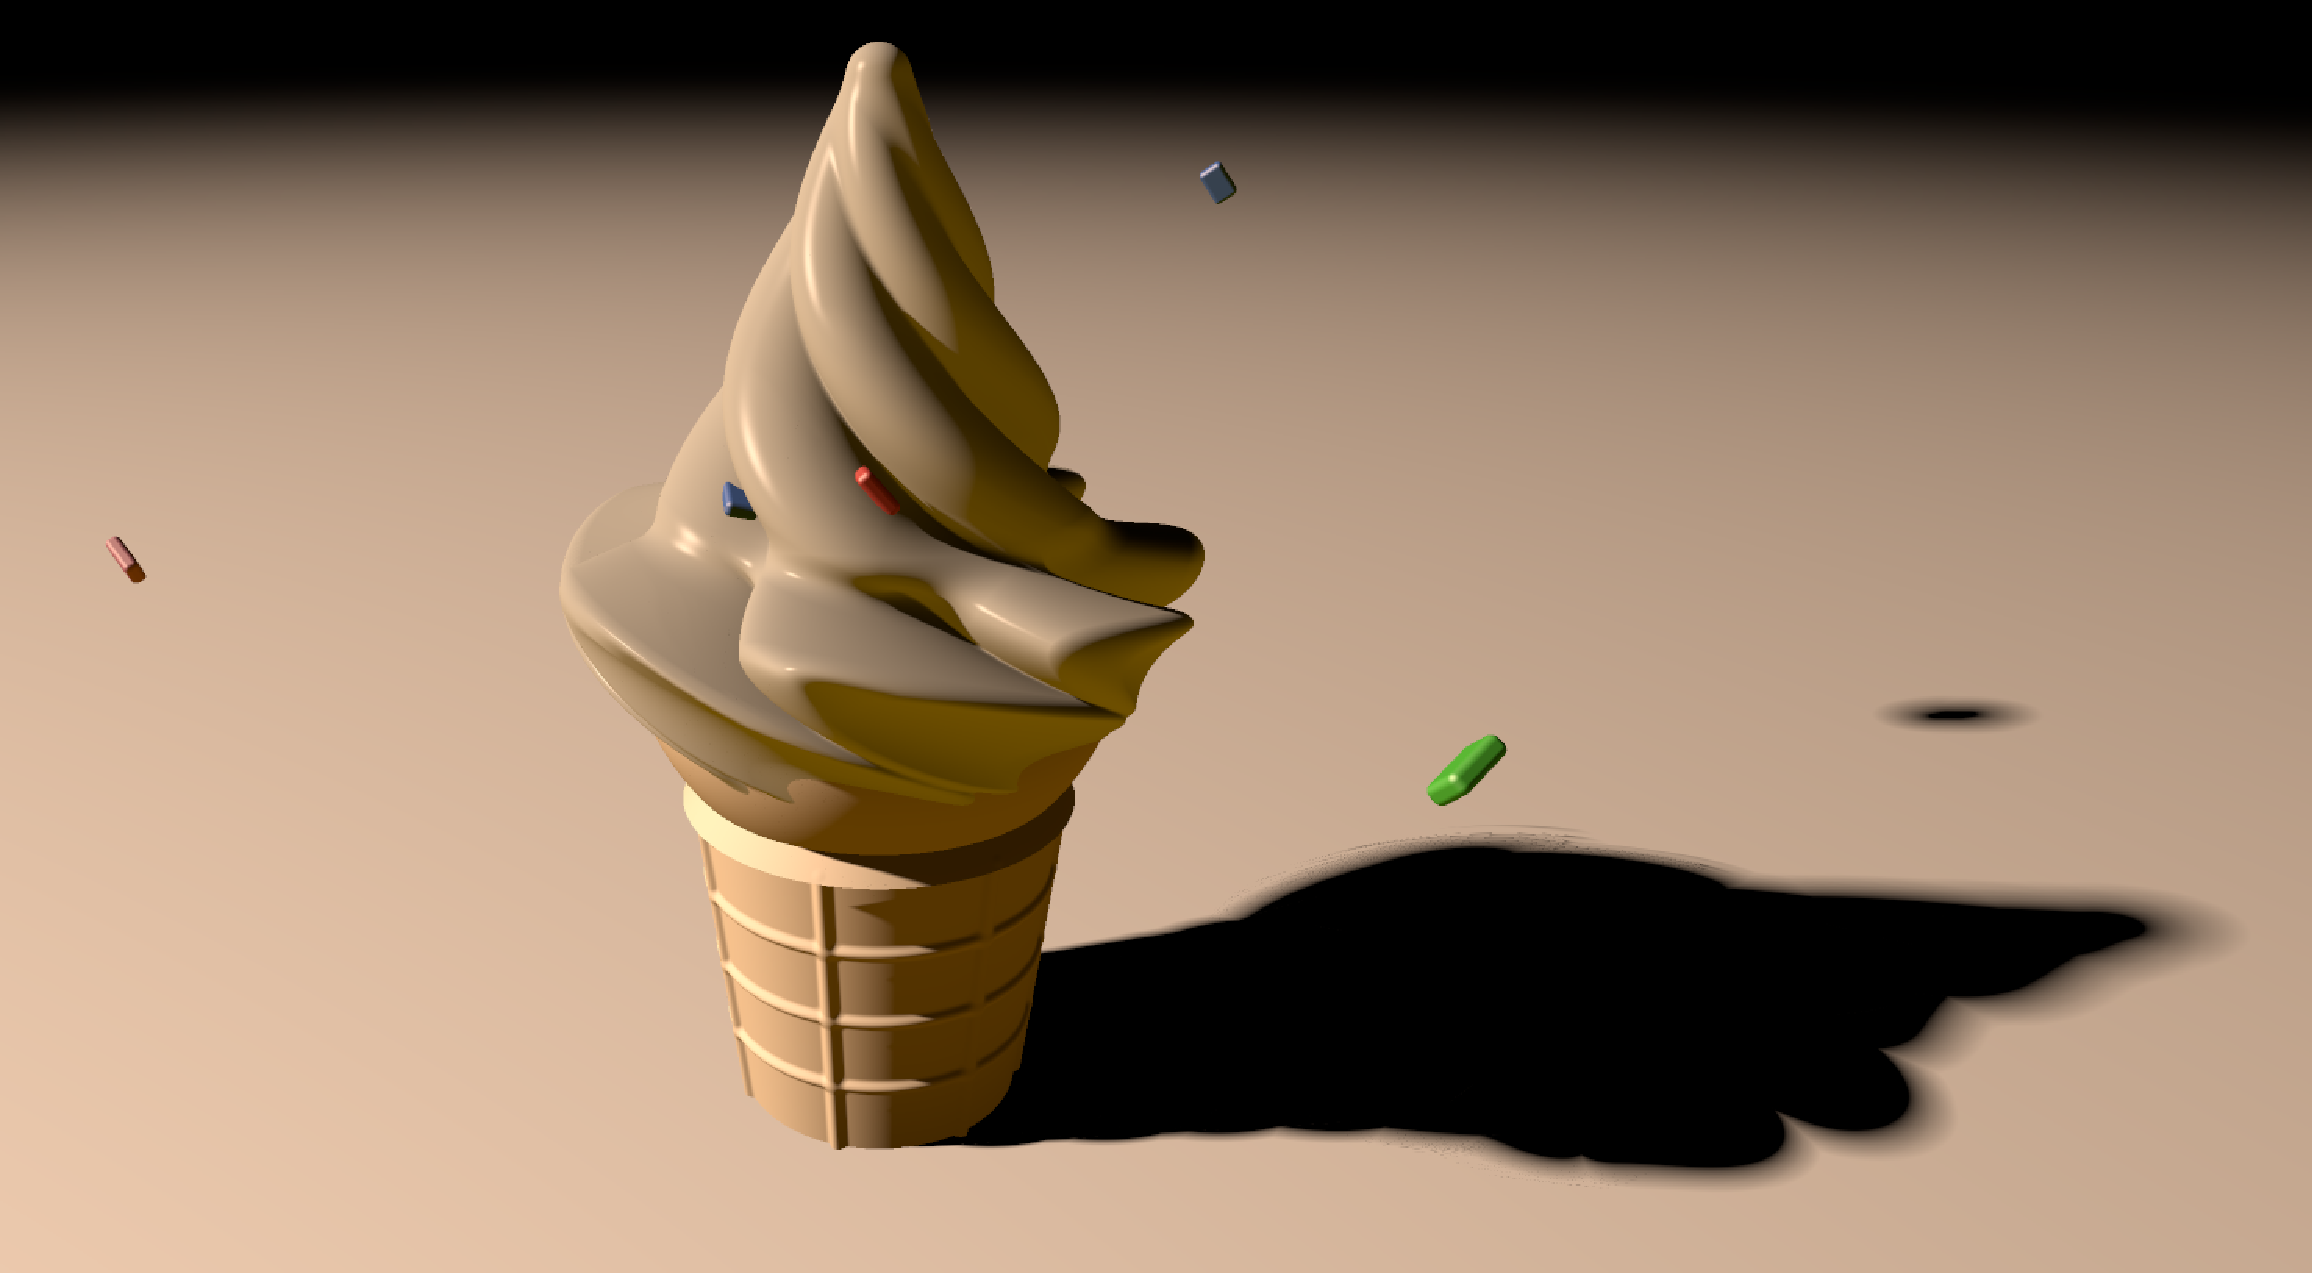
\includegraphics[height=.75\textheight]{images/pre/full.pdf}
        \caption{\url{https://blurgy.xyz/cg/demo.mp4}}
        \label{fig:full}
    \end{figure}
\end{frame}

\begin{frame}
    \frametitle{基本思想}
    \begin{itemize}[<+->]
        \item 用两个直角三角形覆盖整个屏幕
        \item 在片段着色器中构建距离场 (signed distance function, sdf) % 法线方向估计, 物体内部距离为负
        \item 使用 ray march 方法逐像素渲染 % adaptive epsilon
    \end{itemize}
    \begin{figure}[htbp]
        \centering
        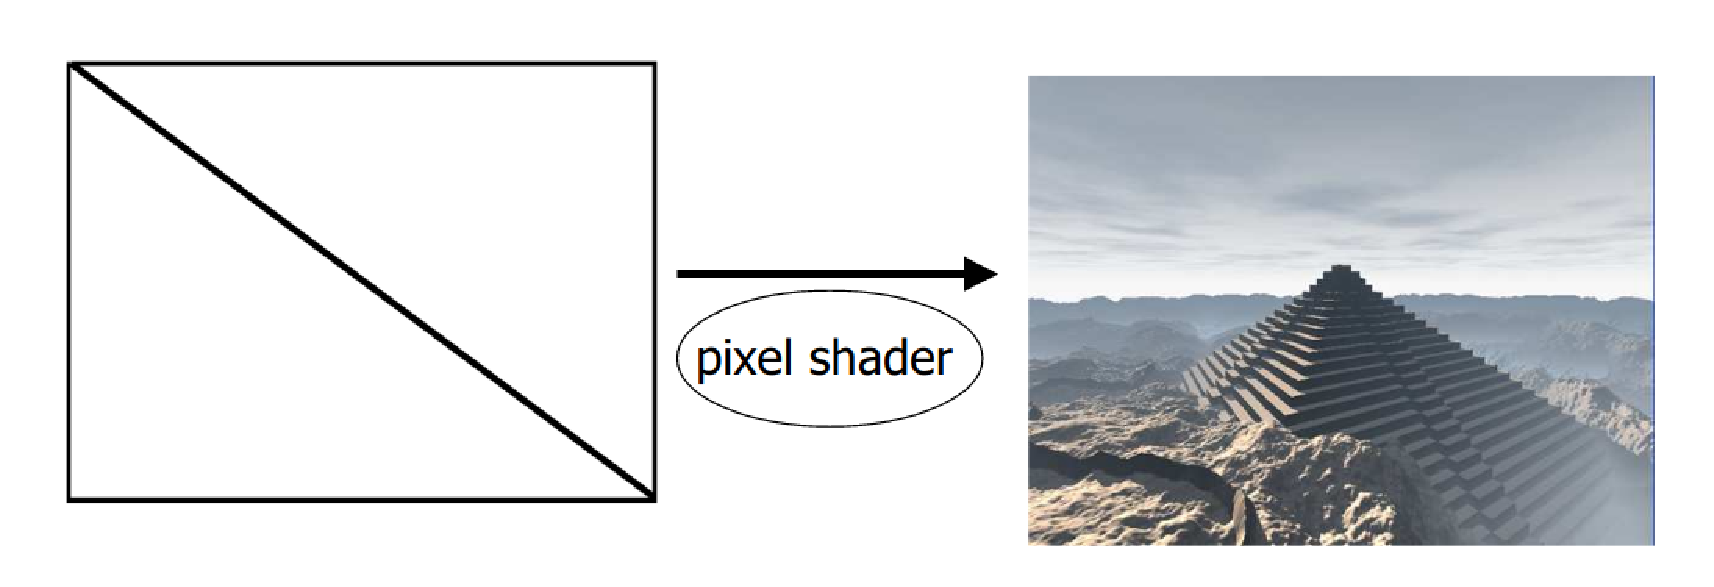
\includegraphics[height=.5\textheight]{images/pre/iq_2tri.pdf}
        \caption{\footnotesize 图片来自 \url{https://www.iquilezles.org/www/material/nvscene2008/rwwtt.pdf}}
        \label{fig:iq_2tri}
    \end{figure}
\end{frame}

\begin{frame}
    \frametitle{目录}
    \tableofcontents
\end{frame}

% TODO: slides 
%************************%
% TODO: fill section (subsection, subsubsection) title here
\section{距离场}
\subsection{甜筒}
% \subsubsection*{}
\begin{frame}
    \frametitle{甜筒 - 分解} % frame title
    \begin{columns}
    \begin{column}{.1\textwidth}\end{column}
        \begin{column}{.4\textwidth}
            \begin{itemize}
                \item 圆台 $\times 2$
                \item 碗形 $\times 1$
                \item 环 $\times 3$
                \item 竖线 $\times 7$
            \end{itemize}
        \end{column}
        \begin{column}{.5\textwidth}
            
\includegraphics[width=128pt]{images/pre/emoji.pdf}
        \end{column}
    \end{columns}
\end{frame}
\begin{frame}
    \frametitle{圆台} % frame title
    \begin{columns}
    % \begin{column}{.1\textwidth}\end{column}
        \begin{column}{.6\textwidth}
            \begin{itemize}[<+->]
                \item 以 Y 轴为中心对称
                \item \texttt{vec3 q = vec3(length(p.xz), p.y);}
                \item 梯形
            \end{itemize}
        \end{column}
        \begin{column}{.4\textwidth}
            \begin{figure}[htbp]
                \centering
                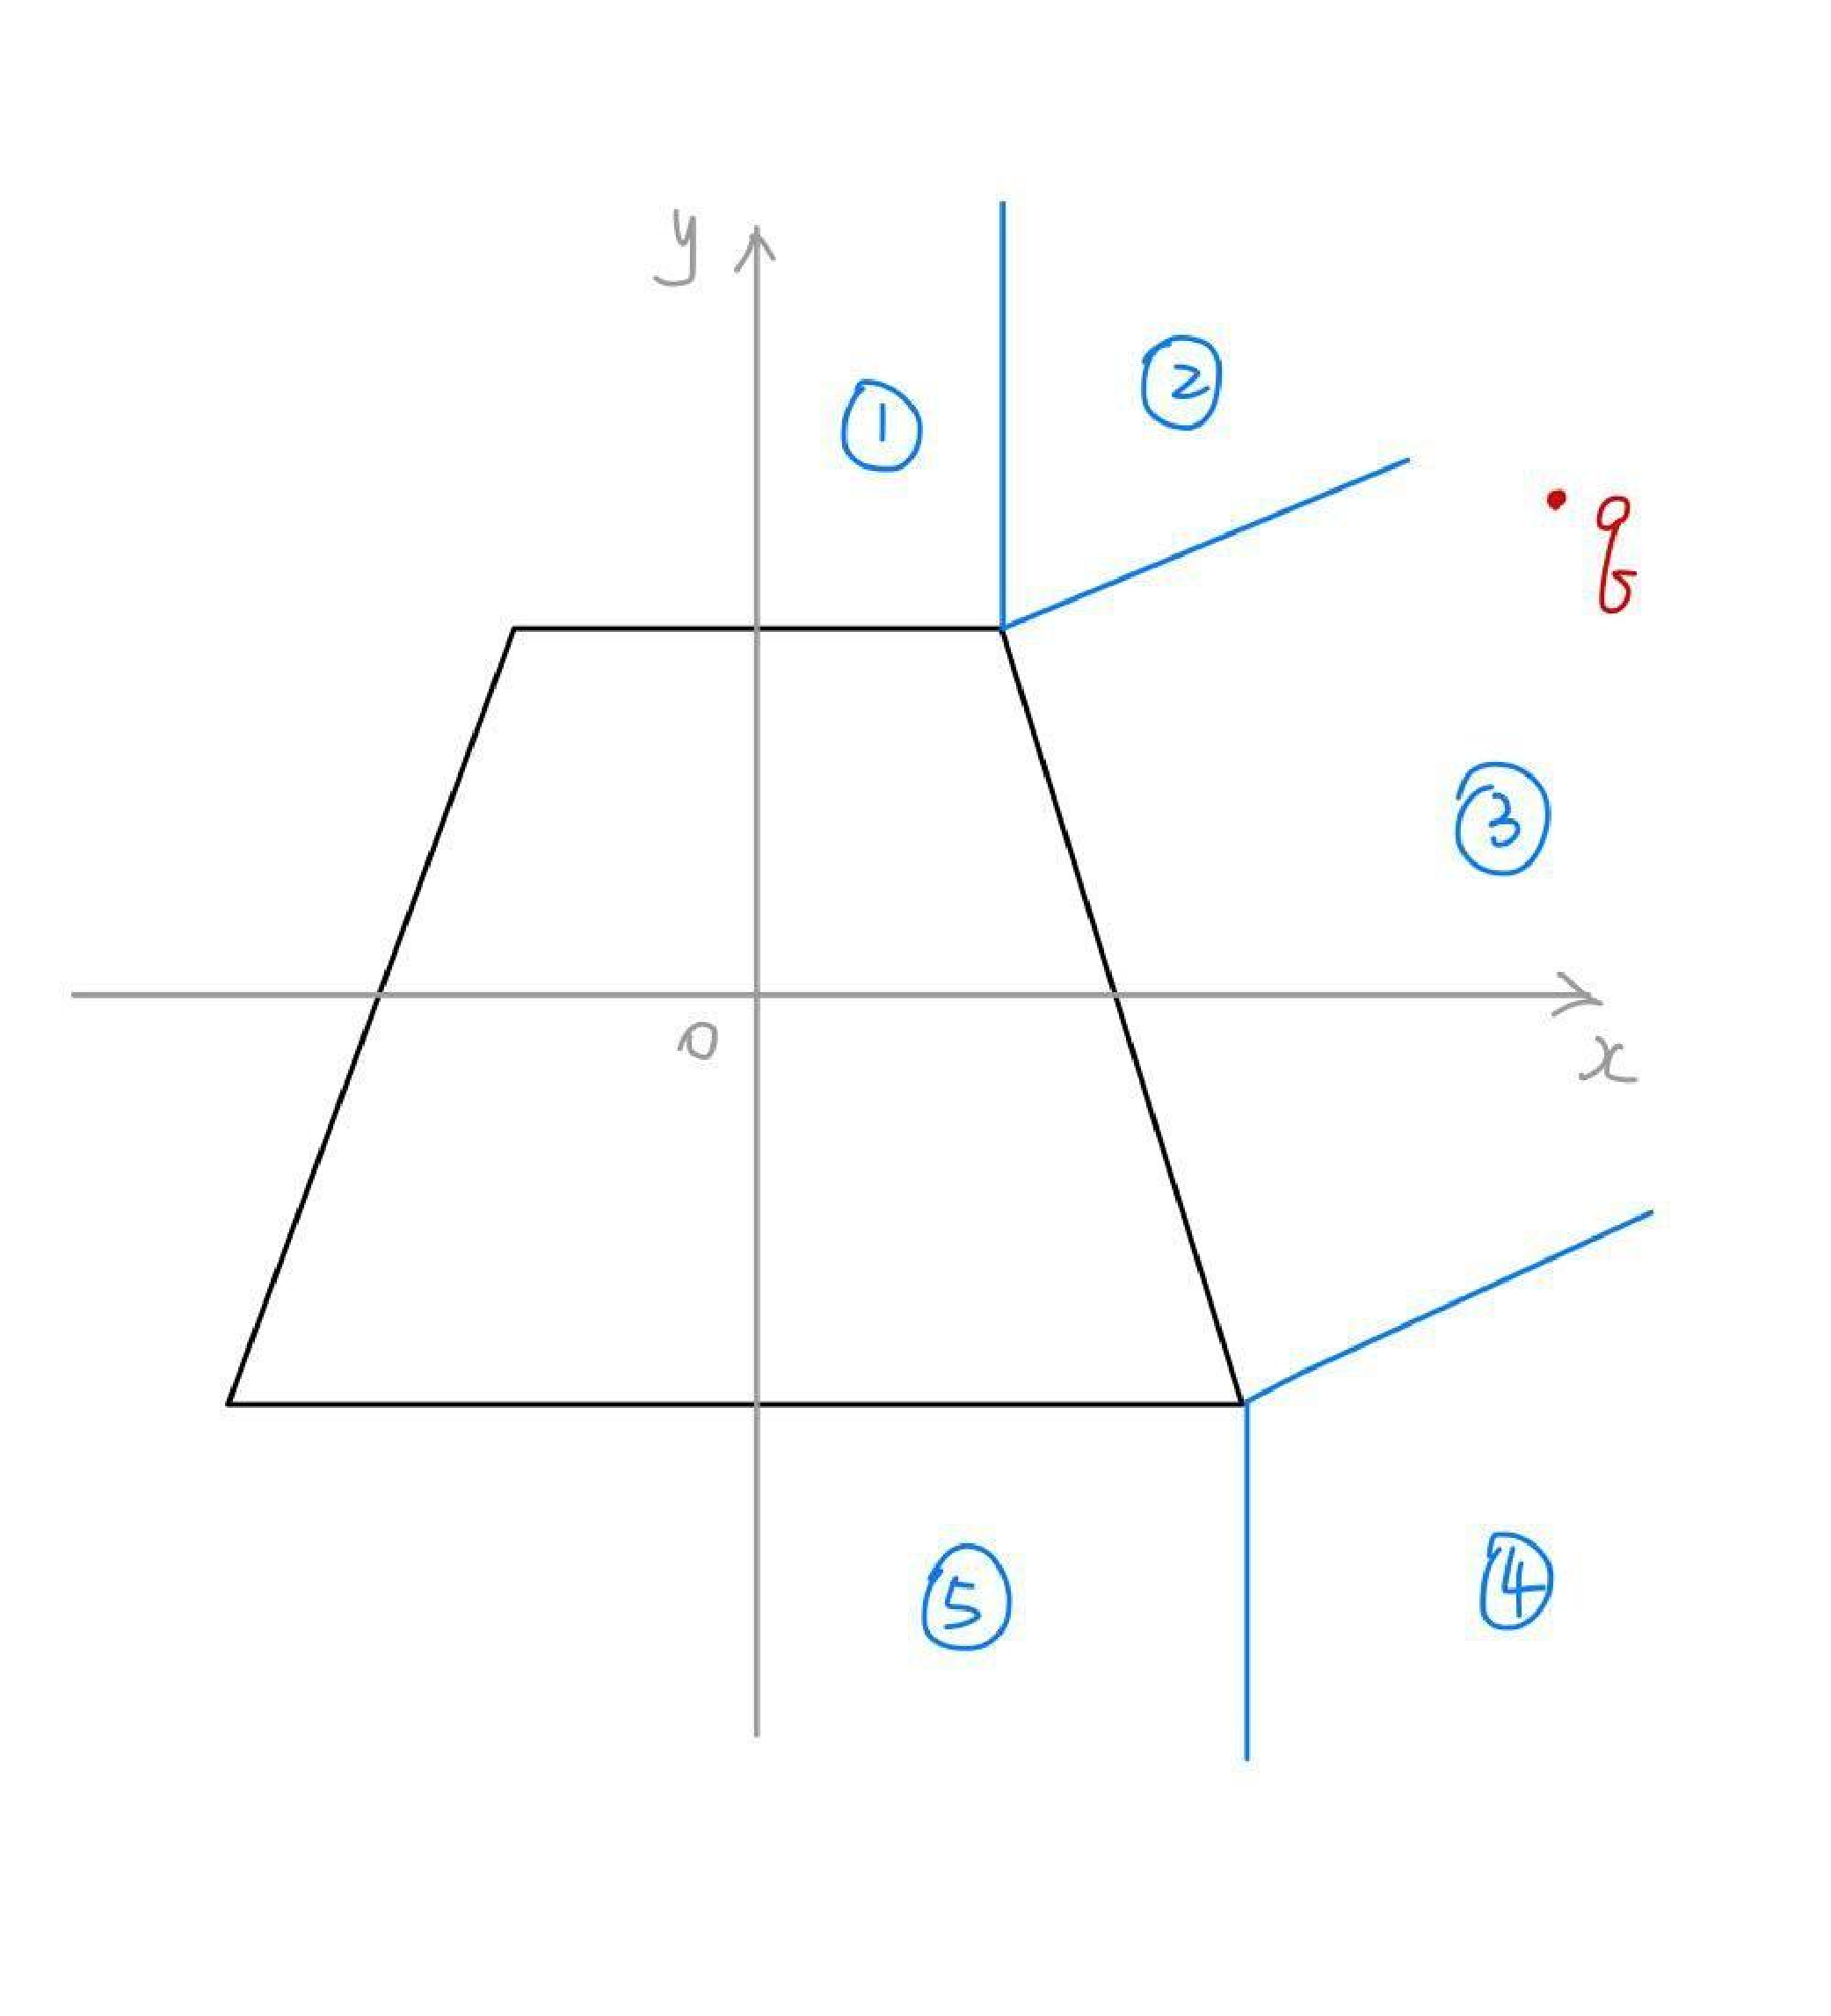
\includegraphics[height=.65\textheight]{images/pre/cone_derive.pdf}
                \caption{}
                \label{fig:cone_derive}
            \end{figure}
        \end{column}
    \end{columns}
\end{frame}
\begin{frame}
    \frametitle{碗形} % frame title
    \begin{columns}
    % \begin{column}{.1\textwidth}\end{column}
        \begin{column}{.6\textwidth}
            \begin{itemize}[<+->]
                \item \texttt{vec3 q = vec3(length(p.xz), p.y);}
                \item 圆 (部分)
            \end{itemize}
        \end{column}
        \begin{column}{.4\textwidth}
            \begin{figure}[htbp]
                \centering
                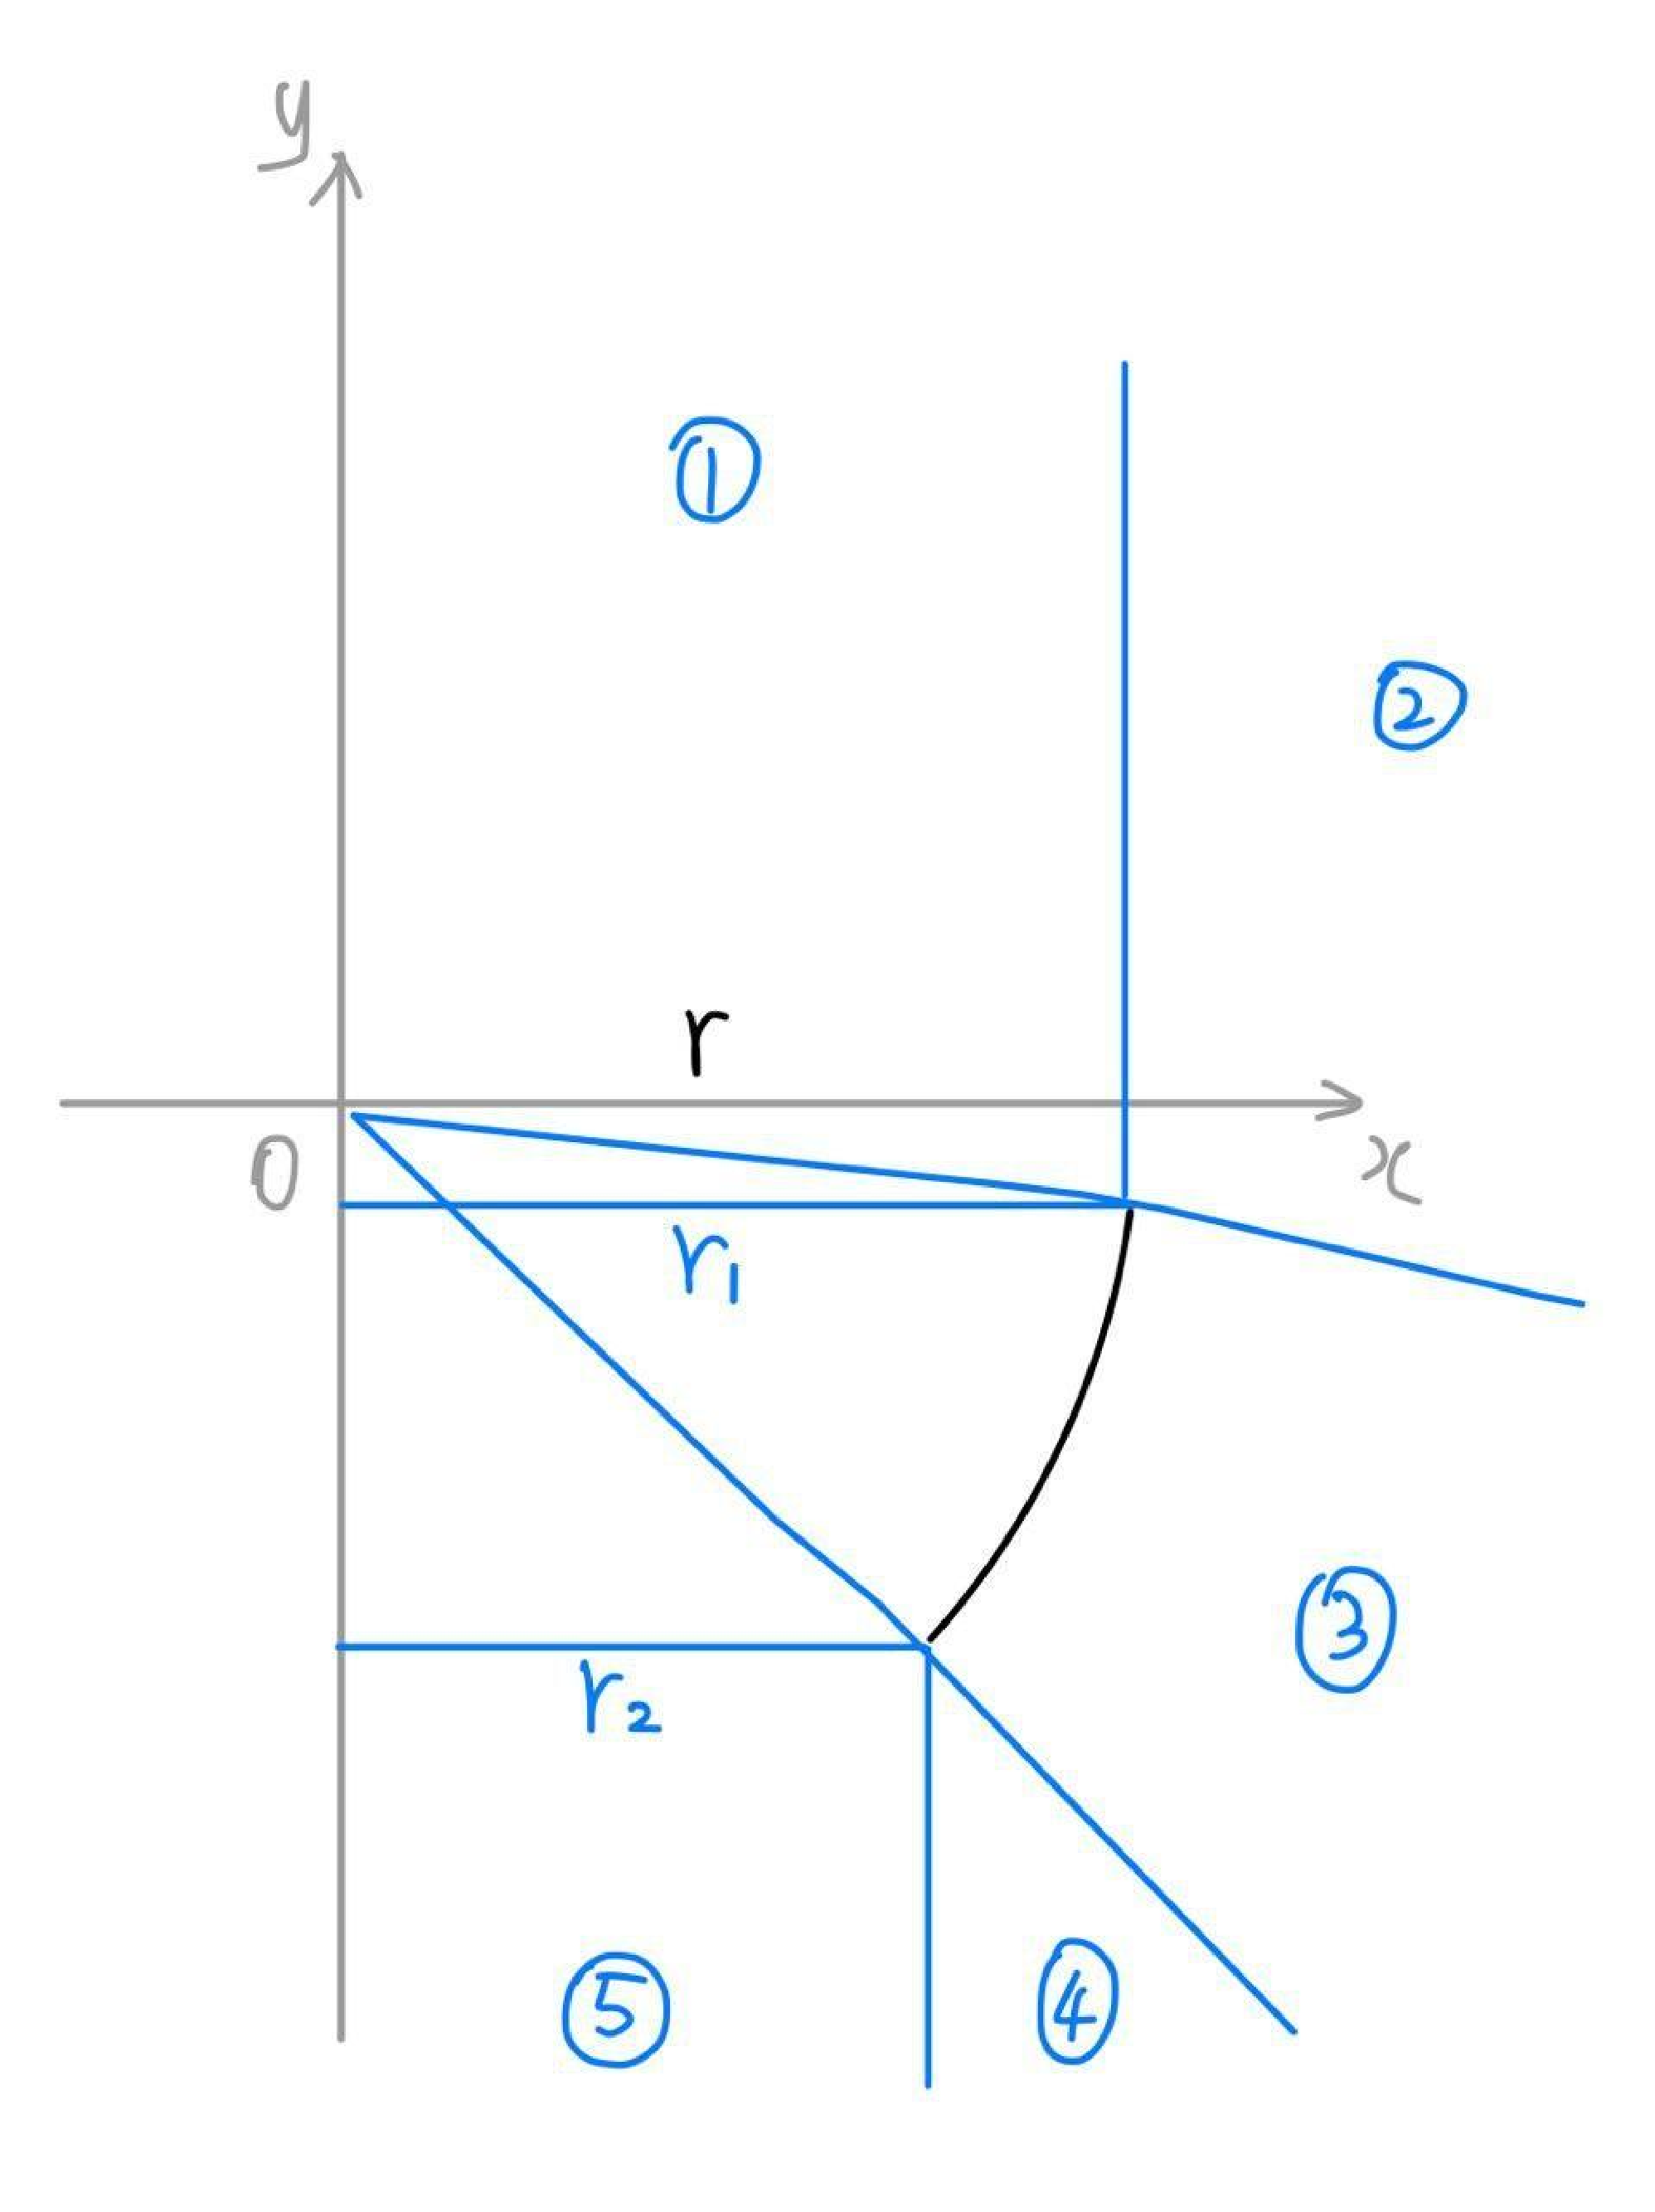
\includegraphics[height=.65\textheight]{images/pre/bowl_derive.pdf}
                \caption{}
                \label{fig:bowl_derive}
            \end{figure}
        \end{column}
    \end{columns}
\end{frame}
\begin{frame}
    \frametitle{五个部分}
    \begin{figure}[htbp]
        \centering
        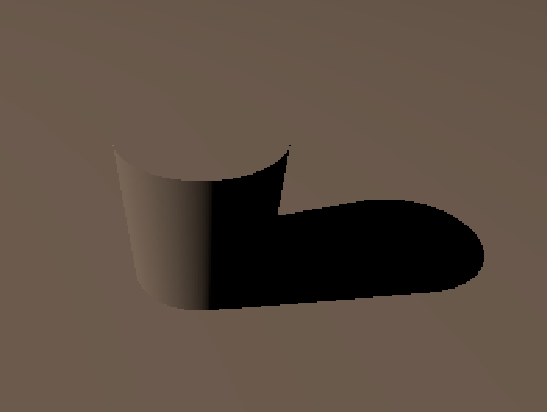
\includegraphics[height=.33\textheight]{images/pre/cone/cone1.pdf}
        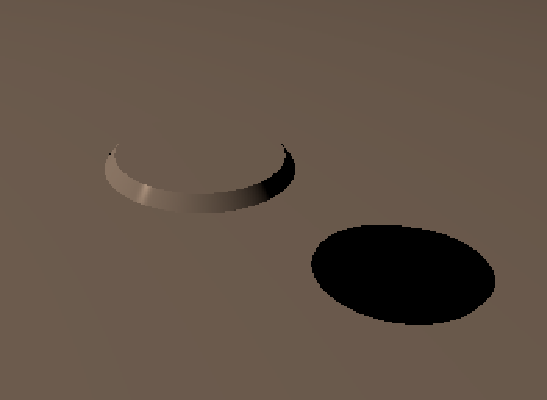
\includegraphics[height=.33\textheight]{images/pre/cone/cone2.pdf}
        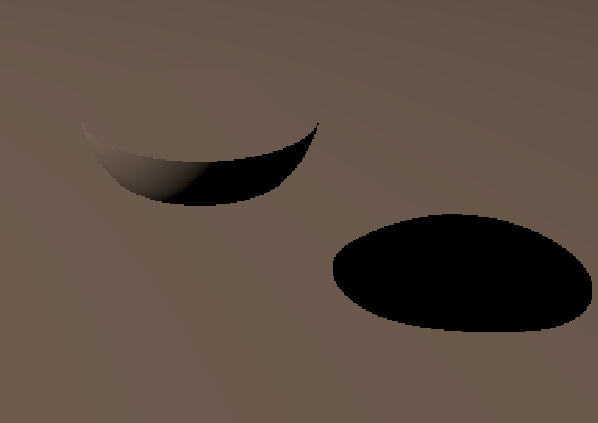
\includegraphics[height=.33\textheight]{images/pre/cone/bowl.pdf}
        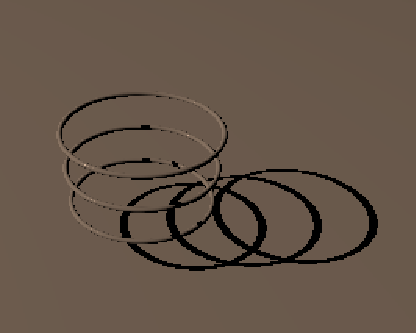
\includegraphics[height=.33\textheight]{images/pre/cone/rings.pdf}
        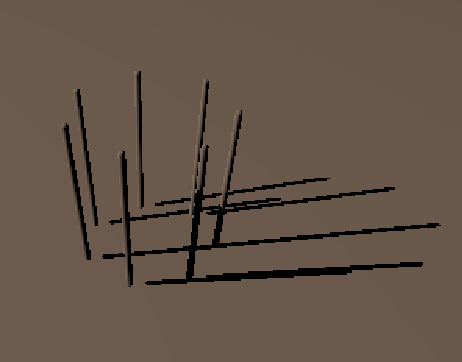
\includegraphics[height=.33\textheight]{images/pre/cone/bars.pdf}
        \caption{}
        \label{fig:cone_parts}
    \end{figure}
\end{frame}
\begin{frame}
    \frametitle{组合}
    \begin{figure}[htbp]
        \centering
        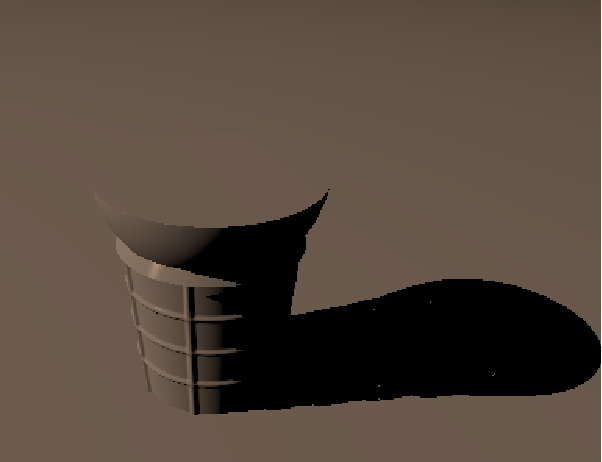
\includegraphics[height=.75\textheight]{images/pre/cone/final.pdf}
        \caption{甜筒}
        \label{fig:cone_model}
    \end{figure}
\end{frame}
%************************%
\subsection{奶油}
\begin{frame}
    \frametitle{奶油 - 分解} % frame title
    \begin{columns}
    \begin{column}{.1\textwidth}\end{column}
        \begin{column}{.4\textwidth}
            \begin{itemize}
                \item 辐射状排列的锥形
                \item 分两层
                \item smooth blending % 模拟奶油
            \end{itemize}
        \end{column}
        \begin{column}{.5\textwidth}
            
\includegraphics[width=128pt]{images/pre/emoji.pdf}
        \end{column}
    \end{columns}
\end{frame}
\begin{frame}
    \frametitle{锥形}
    \begin{itemize}[<+->]
        \item 顶部半径为 0 的\underline{圆台}
        \item \texttt{dist\_cone = CappedCone(h, EPS, r);}
        \item 平滑边缘: \\
        \texttt{dist\_cone = CappedCone(h, EPS, r) - corner;}
    \end{itemize}
\end{frame}
\begin{frame}
    \frametitle{旋转重复}
    \begin{itemize}[<+->]
        \item 变换自身位置以求得不同的距离场
        \item \texttt{vec3 q = rotateY(p, TWOPI*i/rep);} \\ 
        \texttt{dist = min(dist, Cone(q, h, r));}
    \end{itemize}
\end{frame}
\begin{frame}
    \frametitle{两层奶油}
    \begin{block}{下层}
        \begin{figure}[htbp]
            \centering
            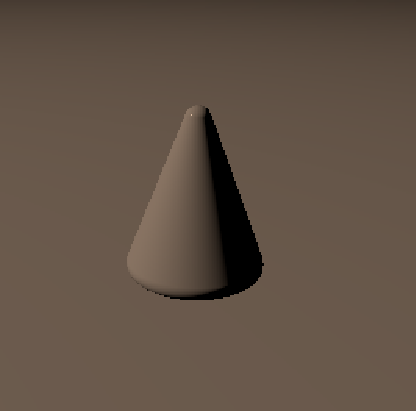
\includegraphics[height=.3\textheight]{images/pre/head/cream1-1.pdf}
            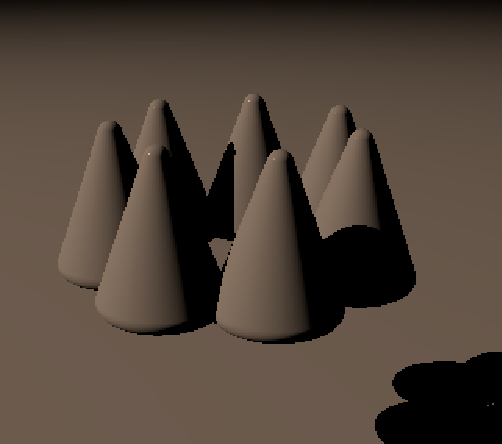
\includegraphics[height=.3\textheight]{images/pre/head/cream1-2.pdf}
            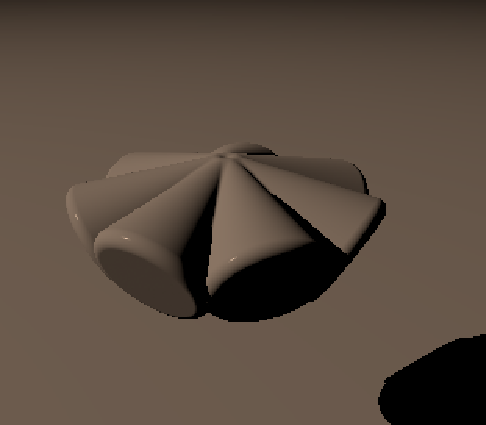
\includegraphics[height=.3\textheight]{images/pre/head/cream1-3.pdf}
            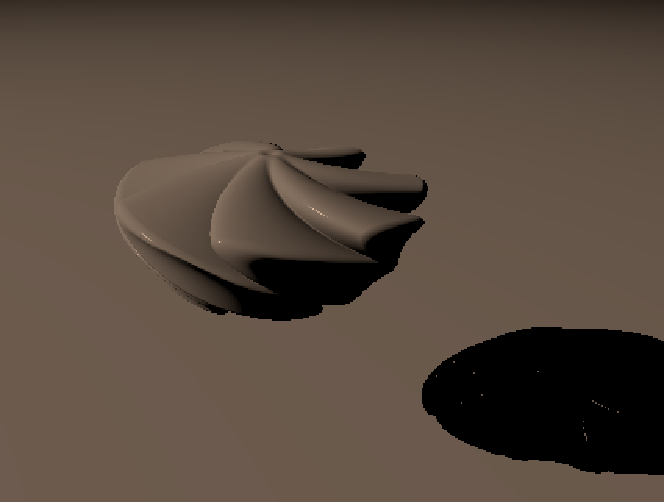
\includegraphics[height=.3\textheight]{images/pre/head/cream1-4.pdf}
            \caption{}
            \label{fig:lower_cream}
        \end{figure}
    \end{block}
    \begin{block}{上层}
        \begin{figure}[htbp]
            \centering
            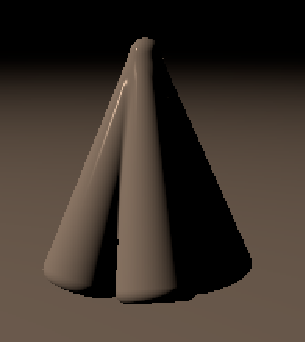
\includegraphics[height=.2\textheight]{images/pre/head/cream2-1.pdf}
            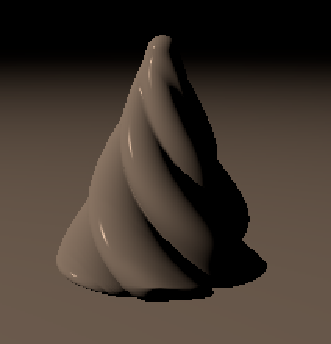
\includegraphics[height=.2\textheight]{images/pre/head/cream2-2.pdf}
            \caption{}
            \label{fig:upper_cream}
        \end{figure}
    \end{block}
\end{frame}
\begin{frame}
    \frametitle{组合}
    \begin{figure}[htbp]
        \centering
        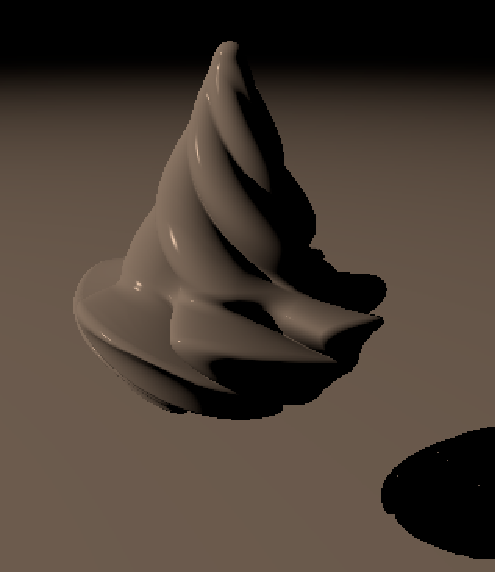
\includegraphics[height=.75\textheight]{images/pre/head/cream.pdf}
        \caption{奶油}
        \label{fig:cream}
    \end{figure}
\end{frame}
\subsection{糖果}
\begin{frame}
    \frametitle{糖果}
    \begin{itemize}
        \item 立方体
        \item 圆角
    \end{itemize}
\end{frame}
\begin{frame}
    \frametitle{旋转}
    \begin{itemize}[<+->]
        \item 随机初始方向
        \item 缓慢旋转
        \begin{itemize}
            \item \texttt{float delta\_rot = 0.07*time + 0.05*sin(time);}
            \item \texttt{vec3 q = inverse(rotateXYZ(ax+delta\_rot, ay, az)) * (p-center);}
            \item \texttt{dist = Box(q, box\_shape);}
        \end{itemize}
    \end{itemize}
\end{frame}
\begin{frame}
    \frametitle{糖果}
    \begin{figure}[htbp]
        \centering
        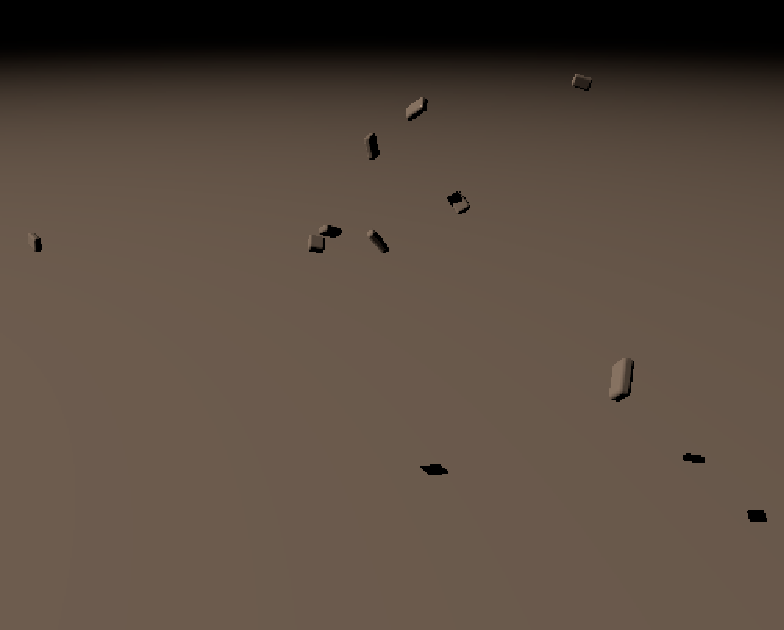
\includegraphics[height=.75\textheight]{images/pre/candies.pdf}
        \caption{糖果}
        \label{fig:candies}
    \end{figure}
\end{frame}
\begin{frame}
    \frametitle{组合}
    \begin{figure}[htbp]
        \centering
        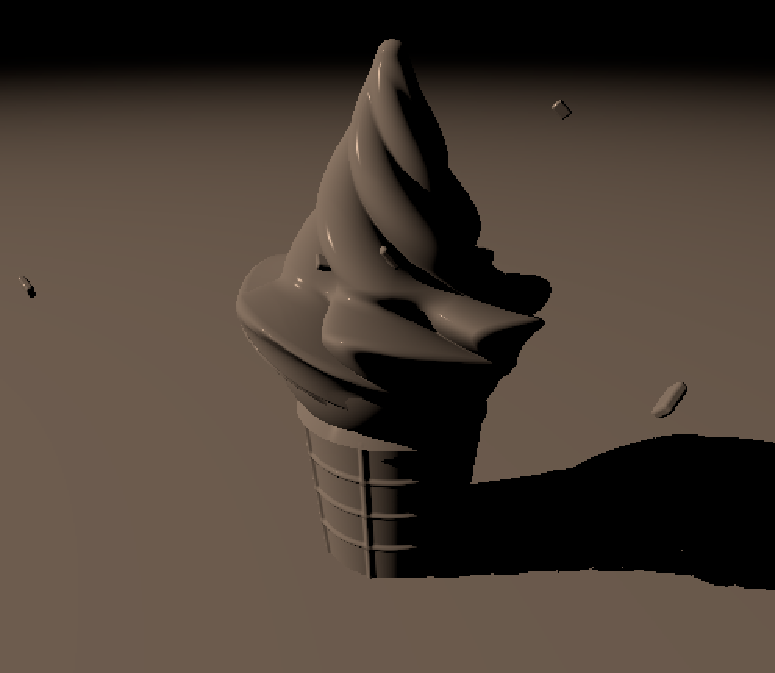
\includegraphics[height=.75\textheight]{images/pre/icecream_model.pdf}
        \caption{\texttt{float dist = mapIceCream(p);}}
        \label{fig:icecream_model}
    \end{figure}
\end{frame}

\section{着色}
\subsection{软阴影}
\begin{frame}
    \frametitle{软阴影估计}
    \begin{itemize}[<+->]
        \item 在光线照亮点 p 的路径上:
        \begin{itemize}
            \item 物体距离路径越近, 阴影越黑
            \item 该物体离 ray marching 的起点越远, 阴影越浅
        \end{itemize}
        \item 物体到起点的距离: \texttt{t}
        \item 物体到 ray marching 路径的距离: \texttt{float h = mapIceCream(ro + t*rd);}
        \item \texttt{k * h / t}
    \end{itemize}
\end{frame}
\begin{frame}
    \frametitle{软阴影}
    \begin{figure}[htbp]
        \centering
        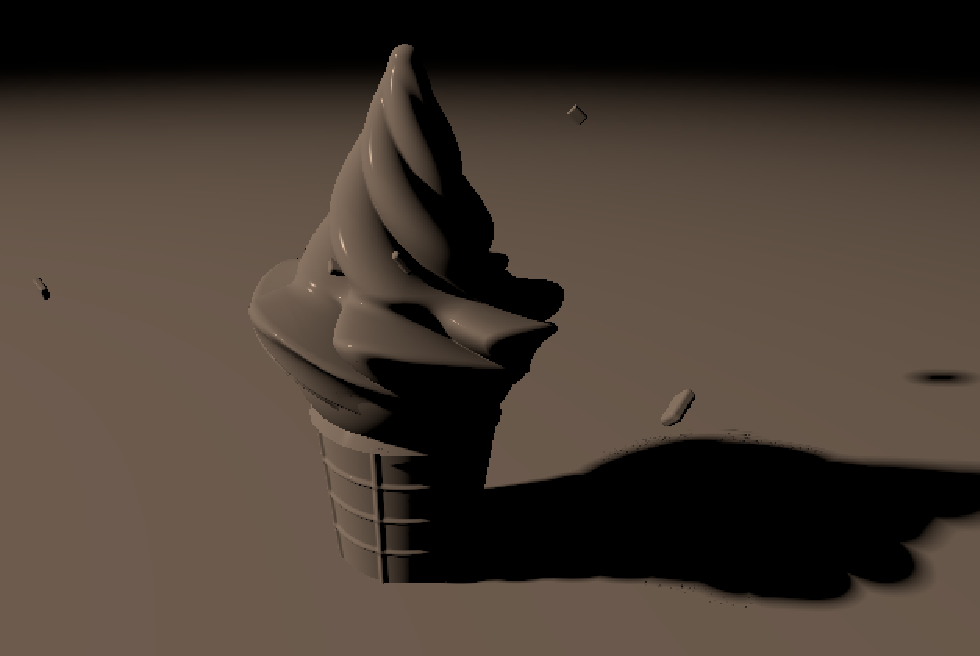
\includegraphics[height=.75\textheight]{images/pre/softshadow.pdf}
        \caption{软阴影}
        \label{fig:softshadow}
    \end{figure}
\end{frame}
\subsection{材质}
\begin{frame}
    \frametitle{材质}
    \begin{itemize}[<+->]
        \item \texttt{Material\{vec3 color; float roughness\}}
        \item \texttt{color}: 漫反射颜色
        \begin{itemize}
            \item \texttt{float diffuse = clamp(dot(n, l), 0, 1) * softShadow(p);}
        \end{itemize}
        \item \texttt{roughness}: 控制高光
        \begin{itemize}
            \item \texttt{float pn = exp2( 10*(1-roughness) );}
            \item \texttt{float specular = pow(clamp(dot(h, n), 0, 1), pn) * diffuse;}
        \end{itemize}
        \item ray marching 过程中更新
    \end{itemize}
\end{frame}
\begin{frame}
    \frametitle{添加材质}
    \begin{figure}[htbp]
        \centering
        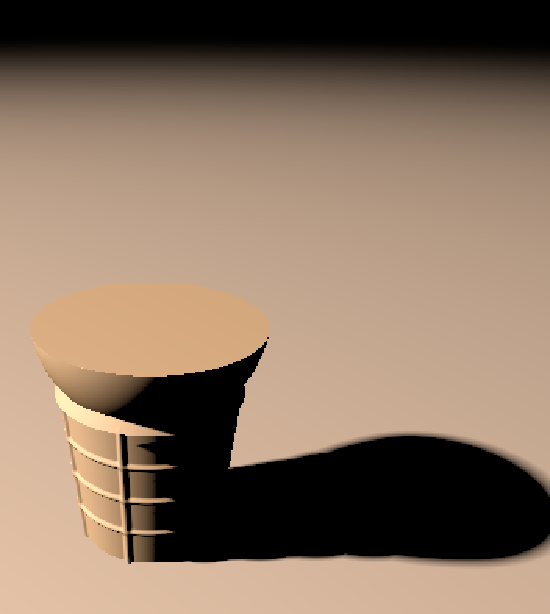
\includegraphics[height=.47\textheight]{images/pre/material/cone.pdf}
        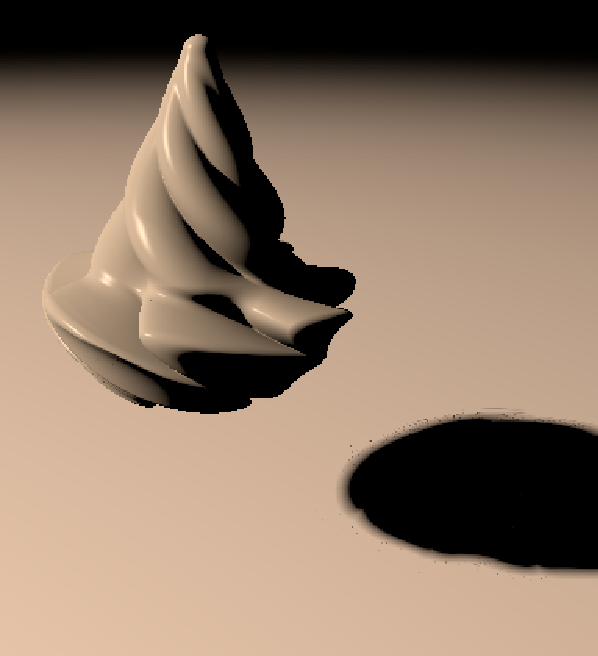
\includegraphics[height=.47\textheight]{images/pre/material/cream.pdf}
        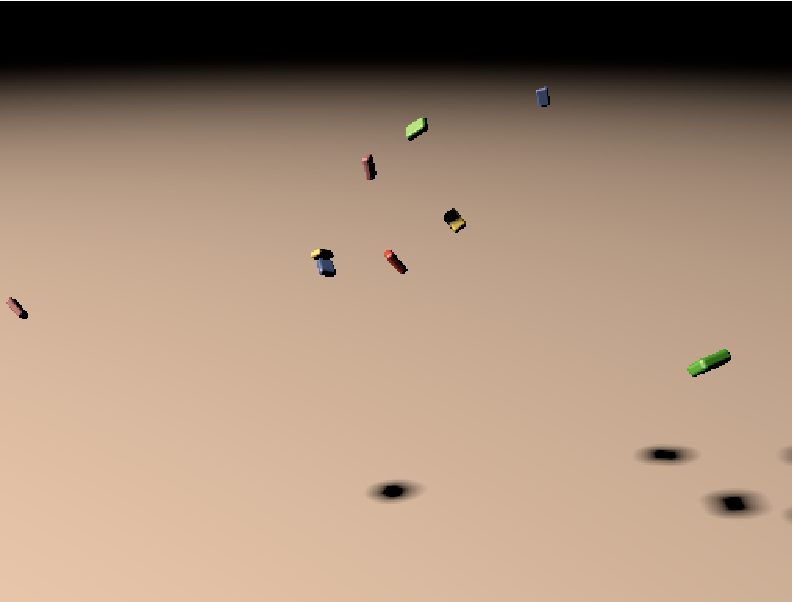
\includegraphics[height=.47\textheight]{images/pre/material/candies.pdf}
        \caption{}
        \label{fig:material_splitted}
    \end{figure}
\end{frame}
\begin{frame}
    \frametitle{组合}
    \begin{figure}[htbp]
        \centering
        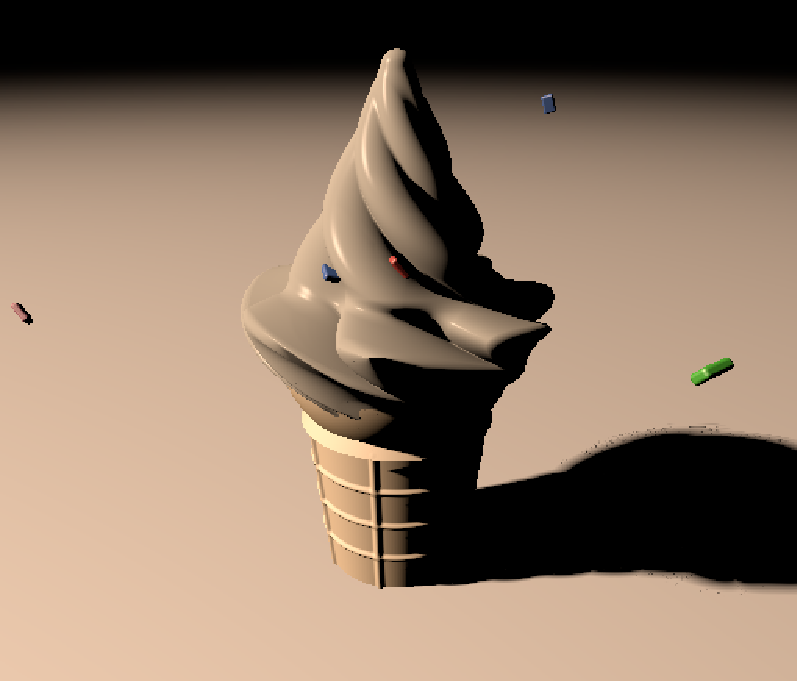
\includegraphics[height=.75\textheight]{images/pre/material/final.pdf}
        \caption{}
        \label{fig:material}
    \end{figure}
\end{frame}

\subsection{环境光照}
\begin{frame}
    \frametitle{环境光遮蔽估计}
    \begin{itemize}[<+->]
        \item 物体表面某点 \texttt{p} 可能因为周围的复杂形状而接收到较少环境光照
        \item 沿表面法线向外取若干个点 \texttt{q} (5 个), 根据 \texttt{q} 点到世界的距离 \texttt{d} 和 \texttt{q} 点到 \texttt{p} 点的距离 \texttt{h}, 估计出点 \texttt{p} 处的遮蔽系数 \texttt{occ}.
    \end{itemize}
\end{frame}

\begin{frame}
    \frametitle{最后}
    \begin{itemize}
        \item 反走样 (SSAA 2x)
    \end{itemize}
\end{frame}

\subsection{最终结果}
\begin{frame}
    \frametitle{最终结果}
    \begin{figure}[htbp]
        \centering
        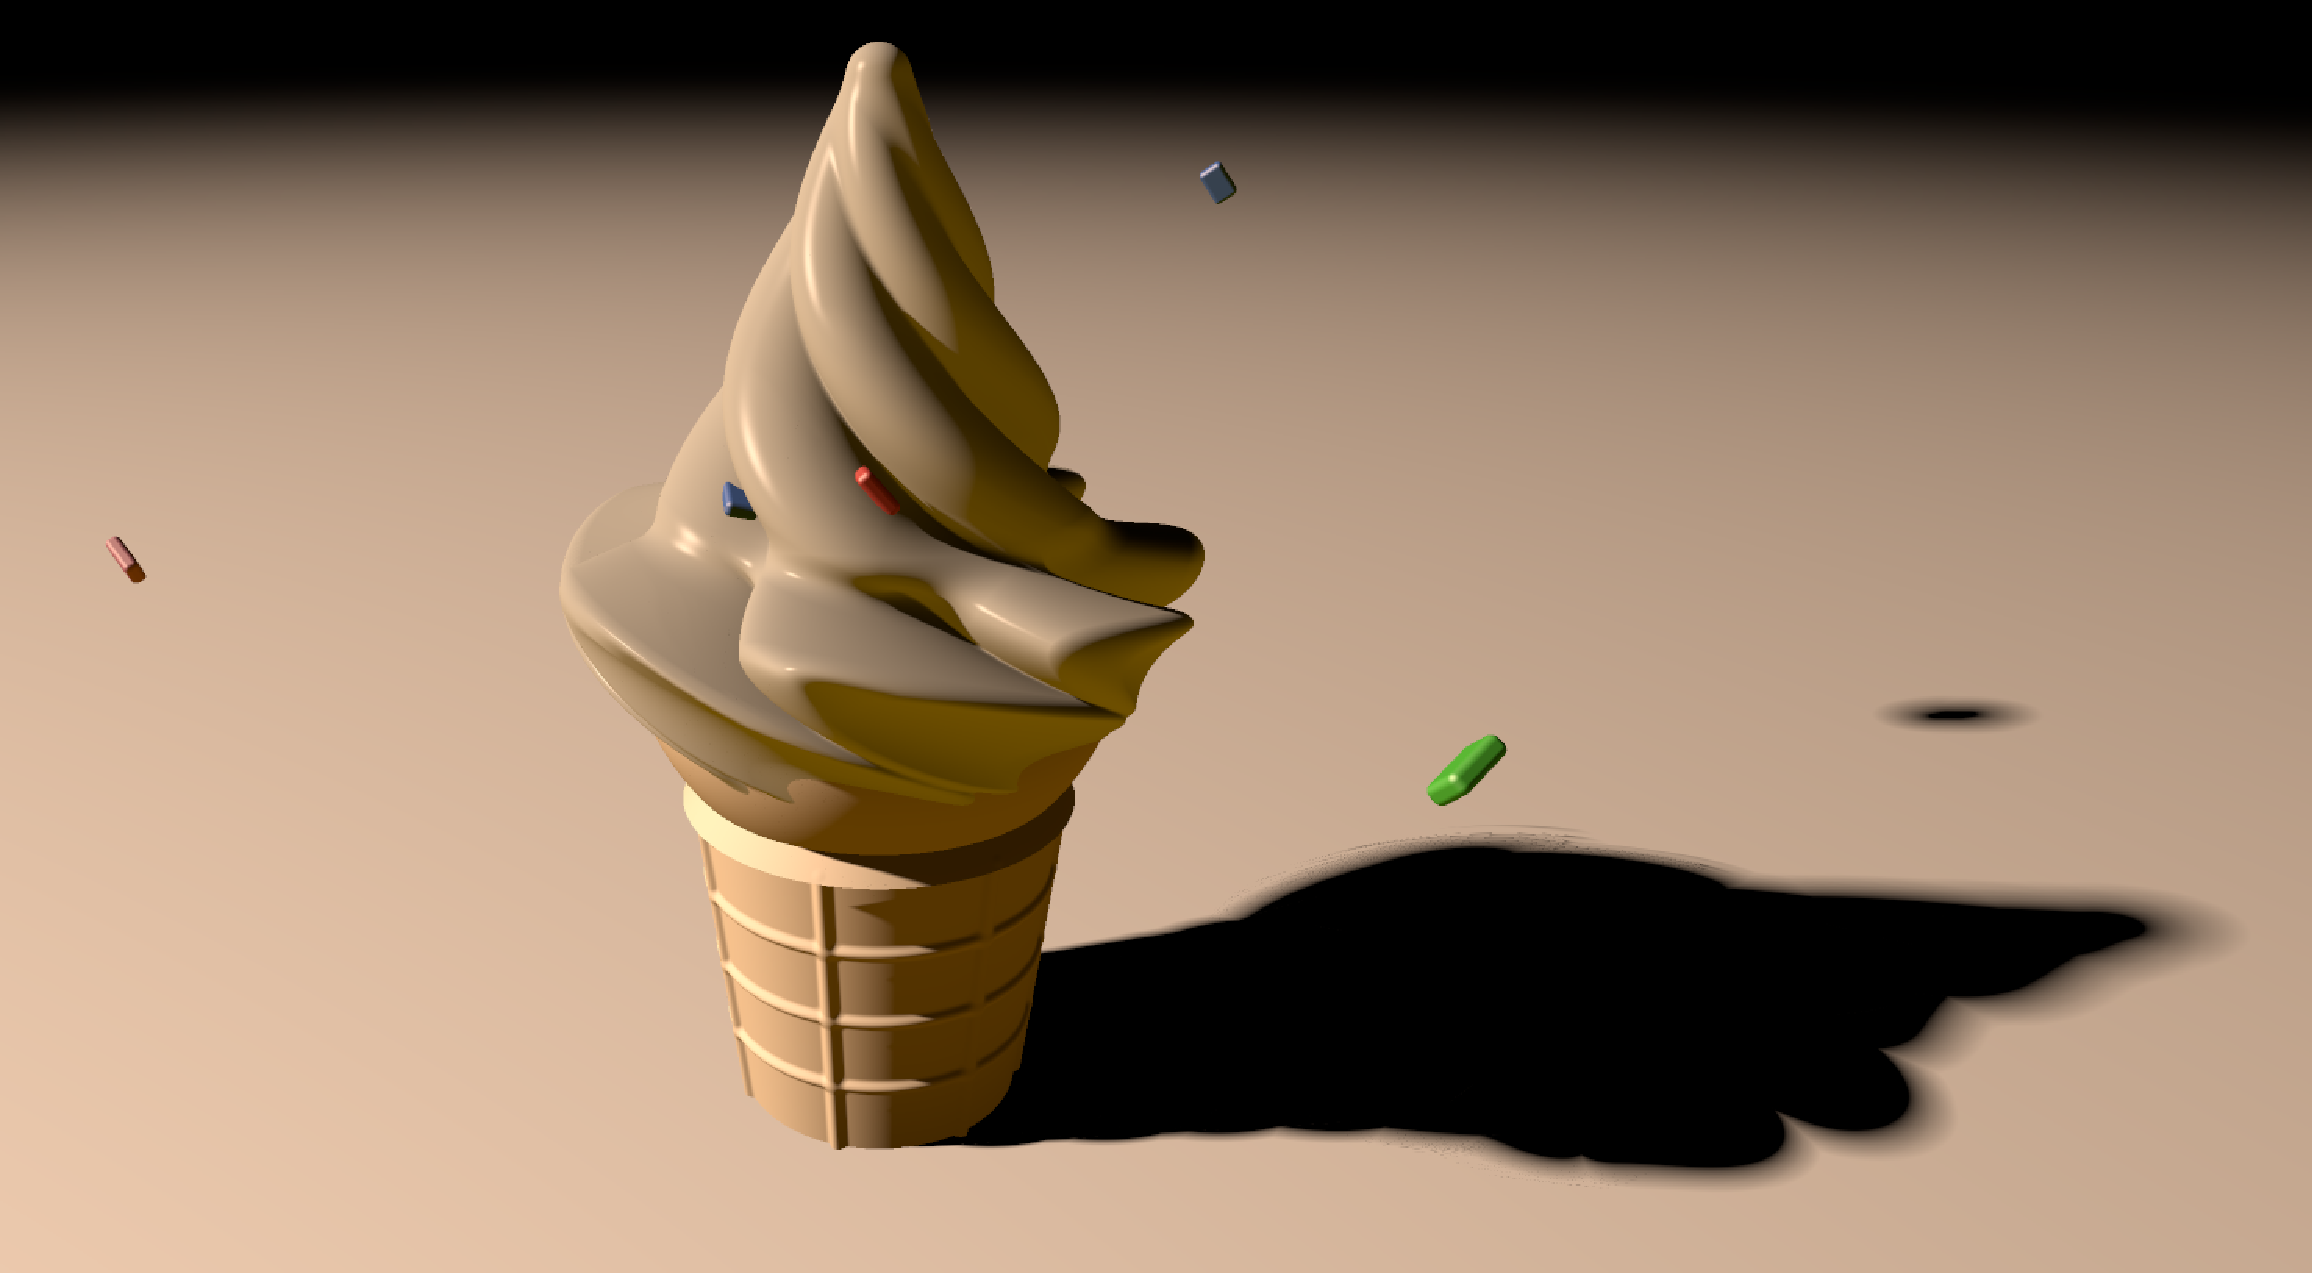
\includegraphics[height=.75\textheight]{images/pre/full.pdf}
        \caption{最终结果}
        \label{fig:final}
    \end{figure}
\end{frame}

\section{参考资料}
\begin{frame}
    \frametitle{参考资料}
    \begin{itemize}
        \item Vulkan API: \url{https://vulkan-tutorial.com/}
        \item ray marching 方法及技巧, 环境光遮蔽估计, 通过空间变换求得绕轴旋转的若干 primitive 等:
        \begin{itemize}
            \item \url{https://www.iquilezles.org/www/material/nvscene2008/rwwtt.pdf} 第 48 页
            \item \url{https://www.youtube.com/watch?v=8sCLZcvC0Oo}
        \end{itemize}
        \item smooth blending: \url{https://iquilezles.org/www/articles/smin/smin.htm}
        \item 修正的圆台距离场函数: \url{https://iquilezles.org/www/articles/distfunctions/distfunctions.htm}
        \item 软阴影估计方式: \url{https://iquilezles.org/www/articles/rmshadows/rmshadows.htm}
    \end{itemize}
\end{frame}

\begin{frame}
    \begin{center}
        \Huge{感谢观看!}
    \end{center}
\end{frame}

\end{document}